\documentclass{article}

\usepackage{geometry}
\usepackage{amsmath}
\usepackage{graphicx, eso-pic}
\usepackage{listings}
\usepackage{hyperref}
\usepackage{multicol}
\usepackage{fancyhdr}
\pagestyle{fancy}
\fancyhf{}
\hypersetup{ colorlinks=true, linkcolor=black, filecolor=magenta, urlcolor=cyan}
\geometry{ a4paper, total={170mm,257mm}, top=10mm, right=20mm, bottom=20mm, left=20mm}
\setlength{\parindent}{0pt}
\setlength{\parskip}{0.3em}
\renewcommand{\headrulewidth}{0pt}

\rfoot{\thepage}
\fancyhf{} % sets both header and footer to nothing
\renewcommand{\headrulewidth}{0pt}
\lfoot{\textbf{CnC Intern Contest}}
\pagenumbering{gobble}

\fancyfoot[CE,CO]{\thepage}
\lstset{
    basicstyle=\ttfamily\small,
    columns=fixed,
    extendedchars=true,
    breaklines=true,
    tabsize=2,
    prebreak=\raisebox{0ex}[0ex][0ex]{\ensuremath{\hookleftarrow}},
    frame=none,
    showtabs=false,
    showspaces=false,
    showstringspaces=false,
    prebreak={},
    keywordstyle=\color[rgb]{0.627,0.126,0.941},
    commentstyle=\color[rgb]{0.133,0.545,0.133},
    stringstyle=\color[rgb]{01,0,0},
    captionpos=t,
    escapeinside={(\%}{\%)}
}

\begin{document}

\begin{center}

    
    \section*{Supir Truk Serakah} % ganti judul soal

    \begin{tabular}{ | c c | }
        \hline
        Batas Waktu  & 5s \\    % jangan lupa ganti time limit
        Batas Memori & 256MB \\  % jangan lupa ganti memory limit
        \hline
    \end{tabular}
\end{center}

\subsection*{Deskripsi}
Loid adalah seorang supir truk yang serakah, dia selalu memilih lokasi terjauh agar bayaran yang diterimanya semakin besar. Terdapat N kota dimana Loid ditugaskan dimana terdapat N-1 jalan ke kota-kota lainnya sehingga membentuk sebuah tree. Kota-kota tersebut dinomori dari 1 sammpai N, dengan kota 1 yang sudah mempunyai supplier bahan makanan. \\
Terdapat 2 query yang harus dipenuhi:

\\ 1 x : mendirikan supplier bahan makanan di kota x
\\ 2 x : toko bahan makanan di x perlu stok bahan makanan, sehingga carilah jarak supplier makanan terjauh


\subsection*{Format Masukan}
Baris pertama  input berisi 2 integer $n$ dan $m$ ($2 \leq n \leq 10^5$, $1 \leq m \leq 10^5$), masing-masing adalah jumlah kota dari tree dan jumlah query dari tree. Baris n-1 berikutnya berisi edge dari tree tersebut, baris ke-i berisi 2 integer yaitu $a_i$ dan $b_i$ ($1 \leq a_i, b_i \leq n, a_i \neq b_i$) yang merupakan edge dari tree tersebut.
\\
\\
m baris berikutnya berisi query. Setiap query berisi sepasang integer yaitu $t_i$ dan $v_i$ ($1 \leq t_i \leq 2$, $1 \leq v_i \leq n$). Jika $t_i$ = 1, maka program harus mendirikan supplier bahan makanan di kota $v_i$. Jika $t_i$ = 2, maka program harus mencari jarak supplier bahan makanan terjauh dari kota $v_i$.
\subsection*{Format Keluaran}
Tuliskan satu baris yang berisi total seluruh query 2, jika tidak ada query 2 maka tulis 0
\\

\begin{multicols}{2}
\subsection*{Contoh Masukan}
\begin{lstlisting}
3 5
1 2
1 3
2 1
2 2
2 3
1 2
2 3
\end{lstlisting}
\columnbreak
\subsection*{Contoh Keluaran}
\begin{lstlisting}
4
\end{lstlisting}
\vfill
\null
\end{multicols}



\pagebreak

\subsection*{Penjelasan}

\begin{center}

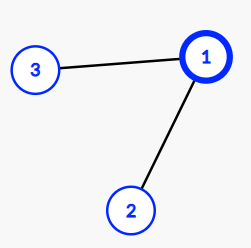
\includegraphics{pertama.PNG}    \\
Peta kota sebelum query. Kota supplier ditandai dengan node yang memiliki warna lebih tebal
\end{center}
query 2 1 = 0 (jarak dari 1 ke 1, karena kota 1 awalnya sudah ada supplier bahan makanan)\\
query 2 2 = 1 (jarak 1 ke 2)\\
query 2 3 = 1 (jarak 1 ke 3)\\
query 1 2 = tambah supplier di kota 2\\

\begin{center}
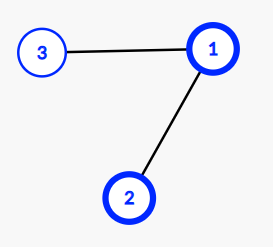
\includegraphics{kedua.PNG}\\
Peta kota setelah query. Terdapat kota supplier baru yaitu kota 2
\end{center}

query 2 3 = 2 (jarak 2 ke 3)\\




\end{document}